\section{Auswertung}
\label{sec:Auswertung}

\subsection{Viskosität von Wasser}

Zunächst wird die Dichte der beiden Kugeln berechnet. Für die Kugeln 
ergaben sich die in Tabelle \ref{tab:Dichte} dargestellten Messwerte für den 
Durchmesser und die Masse, sowie die daraus berechneten Werte für das 
jeweilige Volumen und die Dichte.

\begin{table}
\centering
\caption{Messwerte für Durchmesser, Masse und berechnetes Volumen und Dichte}
\label{tab:Dichte}
\sisetup{table-format=2.1}
\begin{tabular}{c c c c}
\toprule
$d \,/\, \si{\milli\meter}$ & $m \,/\, \si{\gram}$ & $V \,/\, \si{\cm³}$ & $\rho \,/\, \si{\frac{g}{cm³}}$\\
\midrule
15.8 &  5.38 & 2.07 & 2.60\\
15.6 &  4.95 & 1.99 & 2.49\\
\bottomrule
\end{tabular}
\end{table}

Zunächst wurde die Fallzeit der kleinen und großen Kugel bei 21.5°C 
jeweils 10 Mal gemessen. 
Die ermittelten Werte sind in Tabelle \ref{tab:Zeit} aufgetragen. 

\begin{table}
\centering
\caption{Messwerte für die Fallzeiten}
\label{tab:Zeit}
\sisetup{table-format=2.1}
\begin{tabular}{c c}
\toprule
$t\: (kleine\: Kugel)\,/\, \si{\second}$ & $t\: (grosse\: Kugel) \,/\, \si{\second}$\\
\midrule
12.47 & 79.95\\
12.53 & 80.32\\
12.33 & 80.27\\
12.29 & 80.10\\
12.12 & 80.04\\
12.38 & 79.84\\
12.46 & 80.15\\
12.53 & 79.18\\
12.46 & 80.15\\
12.41 & 79.92\\
\bottomrule
\end{tabular}
\end{table}

Aus diesen Werten werden Mittelwert und Standardabweichung gebildet.
$t_g$ ist dabei die Fallzeit der großen und $t_k$ die Fallzeit der kleinen
Kugel.

\begin{align*}
t_k &= \SI{12.40+-0.12}{\second}\\
t_g &= \SI{80.00+-0.31}{\second}
\end{align*}

Nun berechnet sich die Viskosität $\eta$ des Wassers nach (\ref{eqn:Viskosität}).
Die Apperaturkonstante der kleinen Kugel ist gegeben mit 

\begin{equation*}
K_k = \SI{0.0764}{\milli\pascal\cubic\centi\meter\per\gram}
\end{equation*}

Mit der Gaußschen Fehlerfortpflanzung

\begin{align*}
\Delta \eta &= \sqrt{\left(\frac{\partial\eta}{\partial t}\right)^2 \cdot \left(\Delta t\right)²}\\
&=\sqrt{\left(K\cdot(\rho_K - \rho_F)\right)²\cdot(\Delta t)²}
\label{eqn:Fehlereta}
\end{align*}

und der Dichte des Wassers 

\begin{equation}
\rho _F = \SI{998.8}{\kilo\gram\per\cubic\meter}
\end{equation}

ergibt sich folgender Wert für die Viskosität $\eta$:

\begin{equation*}
\eta = \SI{0.001413+-0.000014}{\kilo\gram\per(\meter\second)}
\end{equation*}

Aus diesem Wert kann die Apperaturkonstante $K$ der großen Kugel
bestimmt werden. Dafür wird die Formel \ref{eqn:Viskosität} nach 
$K$ umgestellt: 

\begin{equation*}
K = \frac{\eta}{(\rho_K - \rho_F) \cdot t}
\end{equation*}

Mit der Gaußschen Fehlerfortpflanzung

\begin{align*}
\Delta K &= \sqrt{\left(\frac{\partial K}{\partial \eta}\cdot \Delta\eta\right)² + \left(\frac{\partial K}{\partial t}\cdot \Delta t\right)²}\\
&= \sqrt{\left(\frac{1}{(\rho_K - \rho_F)\cdot t}\cdot \Delta\eta\right)² + \left(\frac{-\eta}{(\rho_K - \rho_F)\cdot t²}\cdot \Delta t\right)²}
\end{align*}

ergibt sich für K: 

\begin{equation*}
K = \SI{493.40+-5}{\nano\meter\squared\per\second\squared}
\end{equation*}

\subsection{Temperaturabhängigkeit der Viskosität}

Die für 10 Temperaturen zwischen 21°C und 70°C gemessenen Fallzeiten 
sind in Tabelle \ref{tab:Temperatur} eingetragen.

\begin{table}
\centering
\caption{Temperaturabhängige Fallzeiten und Viskositäten}
\label{tab:Temperatur}
\sisetup{table-format=2.1}
\begin{tabular}{c c c c c c}
\toprule
$T \,/\, \si{\kelvin}$ & $\frac{1}{T} \,/\, \si{\milli\kelvin^{-1}}$& \multicolumn{2}{c}{t \,/\, \si{\second}} & $\overline{t}$ & $\eta \,/\, \si{\gram\per\second\meter}$\\
\midrule
300.15 & 3.33 & 72.00 & 71.18 & 71.59 \pm\:0.41 & 8.16 \pm\:0.006\\
304.15 & 3.29 & 66.13 & 65.47 & 65.80 \pm\:0.33 & 7.50 \pm\:0.005\\
308.15 & 3.25 & 61.93 & 60.90 & 61.42 \pm\:0.52 & 7.00 \pm\:0.007\\
315.15 & 3.17 & 53.89 & 53.58 & 53.74 \pm\:0.16 & 6.12 \pm\:0.003\\
319.65 & 3.13 & 49.50 & 49.77 & 49.64 \pm\:0.14 & 5.66 \pm\:0.003\\
323.65 & 3.09 & 44.95 & 46.20 & 45.58 \pm\:0.63 & 5.18 \pm\:0.007\\
328.15 & 3.05 & 43.30 & 43.16 & 43.23 \pm\:0.07 & 4.93 \pm\:0.002\\
333.15 & 3.00 & 40.30 & 40.29 & 40.30 \pm\:0.01 & 4.60 \pm\:0.002\\
338.15 & 2.96 & 38.43 & 37.80 & 38.11 \pm\:0.32 & 4.34 \pm\:0.004\\
343.15 & 2.91 & 36.40 & 36.18 & 36.29 \pm\:0.11 & 4.12 \pm\:0.002\\
\bottomrule
\end{tabular}
\end{table}

In der Tabelle sind die jeweiligen Mittelwerte der Fallzeiten mit deren Standardabweichung
aus den beiden Messungen für eine Temperatur aufgeführt. Außerdem wird die 
jeweilige Viskosität nach Formel (\ref{eqn:Viskosität}) ausgerechnet und deren
Fehler durch die Gaußsche Fehlerfortpflanzung nach (\ref{eqn:Fehlereta}) berechnet. 

Nun wird $ln(\eta)$ gegen $1/T$ in Abbildung \ref{fig:plot} aufgetragen.

\begin{figure}
  \centering
  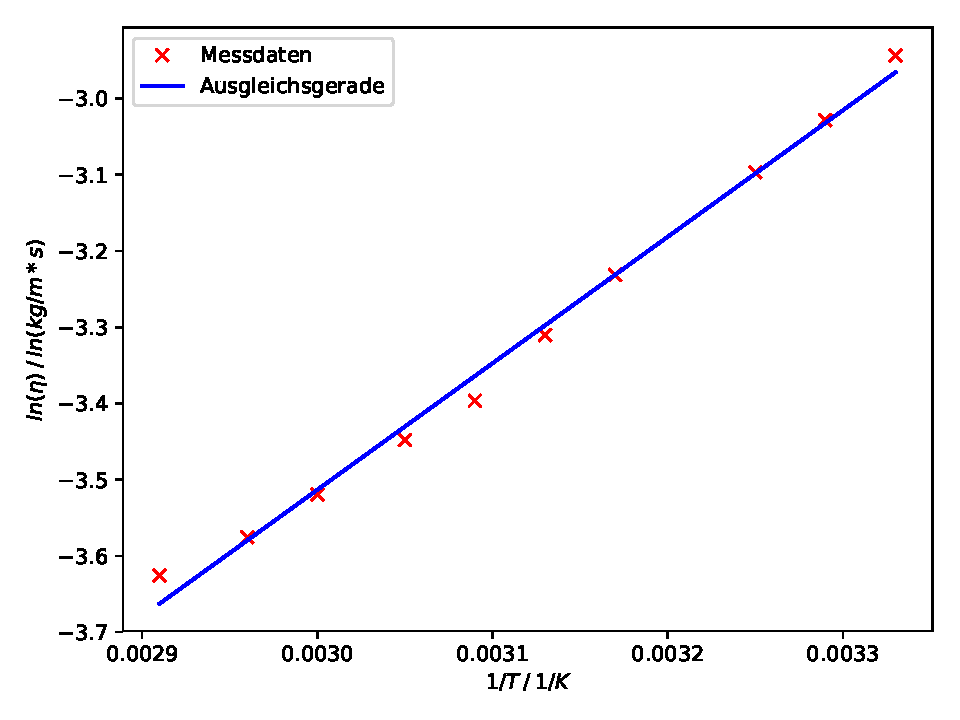
\includegraphics[scale=0.7]{content/plot1.pdf}
  \caption{Temperaturabhängigkeit der Viskosität}
  \label{fig:plot}
\end{figure}

Die lineare Regression, durchgeführt mit Python und Numpy, 
liefert folgende Geradengleichung: 

\begin{equation}
\ln{\eta} = B\cdot \frac{1}{T} + \ln{A}
\end{equation}

Dabei ergeben sich die Parameter zu: 

\begin{align*}
A &= \exp{(-10.353\pm0.1742)} = (\num{3.19e-5}\pm\num{5.56e-6})\si{\kilo\gram\per\meter\per\second} \\
B &= \SI{1658.432+-55.8256}{\kelvin}
\end{align*}

Für die Zeitabhängigkeit der Viskosität gilt also:

\begin{equation}
\eta (T) = (\num{3.19e-5}\pm\num{5.56e-6})\si{\kilo\gram\per\meter\per\second} \cdot \exp{\left(\frac{\SI{1658.432+-55.8256}{\kelvin}}{T}\right)}
\end{equation}

\subsection{Reynolds Zahl}

Mit den berechneten Werten lässt sich nun die Reynoldszahl für die 
jeweiligen Temperaturen berechnen. Die Ergebnisse für die große Kugel sind 
in Tabelle \ref{tab:Zeit} aufgeführt.

\begin{table}
\centering
\caption{Temperaturabhängige Reynoldszahl}
\label{tab:Zeit}
\sisetup{table-format=2.1}
\begin{tabular}{c c c}
\toprule
$T\,/\, \si{\kelvin}$ & $v\,/\, \si{\milli\meter\per\second}$ &$Re$\\
\midrule
300.15 & 1.397 \pm\:0.008 &  27.02\pm\:0.16\\
304.15 & 1.520 \pm\:0.008 &  31.98\pm\:0.17\\
308.15 & 1.682 \pm\:0.014 &  36.70\pm\:0.32\\
315.15 & 1.861 \pm\:0.006 &  47.99\pm\:0.16\\
319.65 & 2.015 \pm\:0.006 &  56.18\pm\:0.17\\
323.65 & 2.199 \pm\:0.030 &  67.00\pm\:0.90\\
328.15 & 2.313 \pm\:0.004 &  74.04\pm\:0.13\\
333.15 & 2.481 \pm\:0.001 &  85.11\pm\:0.05\\
338.15 & 2.624 \pm\:0.022 &  95.40\pm\:0.80\\
343.15 & 2.762 \pm\:0.008 & 105.79\pm\:0.31\\
\bottomrule
\end{tabular}
\end{table}

Außerdem ergibt sich die Reynoldzahl für die kleine Kugel: 

\begin{equation*}
Re_{kl} = \num{890.7+-1.1}
\end{equation*}

Es ist zu erkennen, dass die Reynoldzahlen für alle Temperaturen unter 1160 
liegen und man somit von laminaren Stömungsverhältnissen ausgehen kann.